\chapter{Deep learning}
\label{cha:deep_learning}
A crucial limitation of the perceptron is that it can only model linear functions. Hence, as we have discussed, we cannot for example provide a linear separation for the XOR. We introduced non-linearity by means of feature mapping. Moreover, we studied how to implicitly provide non-linearity via kernels. To do this we need to design appropriate kernels (possibly selecting from a set, i.e. kernel learning) able to produce reasonable similarity measures. The most common solution (i.e. the decision function) is \textit{linear combination of kernels}.
$$f(\pmb{x}) = \sum_i \alpha_i y_i K(\pmb{x_i}, \pmb{x})$$
\textbf{Remark:} this formula is meaningful for the classification case. In regression the coefficient for $K(\pmb{x_i}, \pmb{x})$ is different. \newline

There are two main drawback regarding kernels:
\begin{itemize}
    \item We need to design appropriate kernels, perhaps selecting from a set.
    \item Once the appropriate kernels are selected, the decision function is a linear combination of them. The kernel structure is constant and it is not learned or progressively refined.
\end{itemize}

The \textit{multilayer perceptron} (MLP) is the simplest network of interconnected neurons.  It is a layered architecture: neurons from one layer send outputs to the following layer (this structure is named \textit{feed forward neural network}). The input layer is at the bottom of the architecture (input features). One or more hidden layers are placed in the middle (learned features). Finally on the top there is the output layer (where the prediction takes place). A graphical representation of the multilayer perceptron is illustrated in Figure \ref{fig:mlp}. \newline

\begin{figure}
    \centering
    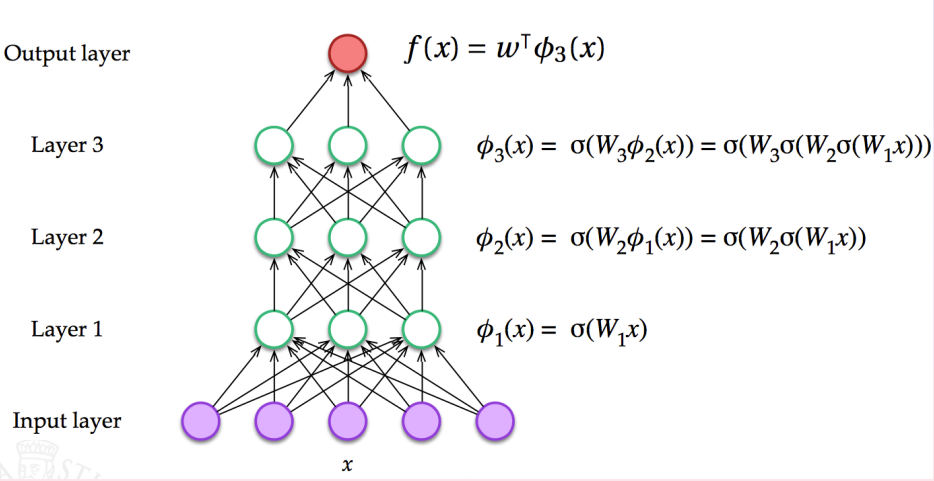
\includegraphics[width=\textwidth]{images/mlp.png}
    \caption{Multilayer Perceptron (MLP)}
    \label{fig:mlp}
\end{figure}

\textbf{Remark:} the neuron in the input layer are not exactly neuron. Indeed, they represent the features of the given input. \newline

\textbf{Remark:} the connections are always from one layer to the following layer. Each neuron has a connection with each of the neurons of the following layer. This structure is called \textit{densely connected architecture}. This is in contrast to the case of convolutional neural networks for example, where the structure of connections is template based. \newline

\textbf{Remark:} on the right of the structure there are the formulas which describe the behaviour of the neural network.
\begin{itemize}
    \item Note that each $W_i$ is a matrix of weights. For example $W_1$ represents the weights of the first layer. Each row of the matrix represents the weights of one neuron in the layer. The weights values are the weights of each input of the given neuron. The product $W_1 \pmb{x}$ returns a vector which is a value for each of the hidden neurons.
    
    \item $\sigma$ is a non linear function called \textit{activation function} which is applied to the weighted sum of the inputs. Overall, the operation in the first layer is represented by $\phi_1(x)$.
\end{itemize}

\textbf{Remark:} a beautiful aspect of this structure is the following:
\begin{itemize}
    \item In non-linear kernel machines the decision function is described by: $$f(\pmb{x}) = w^T \phi(\pmb{x})$$
\end{itemize} In the multilayer perceptron, the final output layer is described by $$f(\pmb{x}) = w^T \phi_3(\pmb{x})$$
However in the case of multilayer perceptron the function $\phi_3(\pmb{x})$ is not fixed but it is learned. Indeed all the weights of the structure are learned. We have not to design a kernel, we delegate to the neural network the task of defining a proper data representation (more flexibility). The downside is that, in order to learn this representation, a lot of data is needed. \newline

\textbf{Remark:} without $\sigma$ the decision function would look like a linear function:
$$f(\pmb{x}) = \pmb{w}^T W_3 W_2 W_1 \pmb{x} = W_{\text{all}}^T \pmb{x}$$

\section{Activation Function}
In Figure \ref{fig:perceptron_activation_function} it is illustrated a single perceptron which is composed of a summation and an activation function. The activation function is the \textit{threshold activation}.
$$f(\pmb{x}) = \mathit{sign}(\pmb{w}^T \pmb{x})$$
The derivative of the function is zero everywhere apart from zero, where it is not differentiable. As a result, it is impossible to run gradient-based optimization. Hence, we cannot minimize the error function, there is not chance to propagate a gradient. In conclusion, the threshold activation is not a valid activation function for a deep neural network. \newline

\begin{figure}
    \centering
    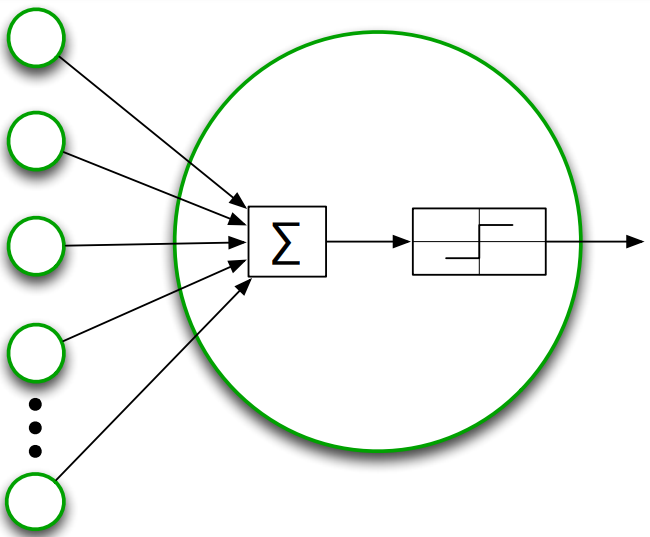
\includegraphics[width=0.7\textwidth]{images/perceptron_activation_function.png}
    \caption{Single perceptron.}
    \label{fig:perceptron_activation_function}
\end{figure}

\textbf{Remark:} $\mathit{sign(x)}$ is equal to +1 if $x$ is positive and $\mathit{sign(x)}$ is equal to -1 if $x$ is negative. This function is clearly non-linear \newline

We need a smoother function. The literature proposed the \textit{sigmoid} function as a reasonable alternative.
\begin{equation}
    f(\pmb{x}) = \sigma(\pmb{w}^T \pmb{x}) = \frac{1}{1+\text{exp}(-\pmb{w}^T \pmb{x})}
\end{equation}
The function is illustrated in Figure \ref{fig:sigmoid}. Actually, the curve is a smooth version of threshold. The behaviour is approximately linear around zero and it saturates for large and small values. \newline

\begin{figure}
    \centering
    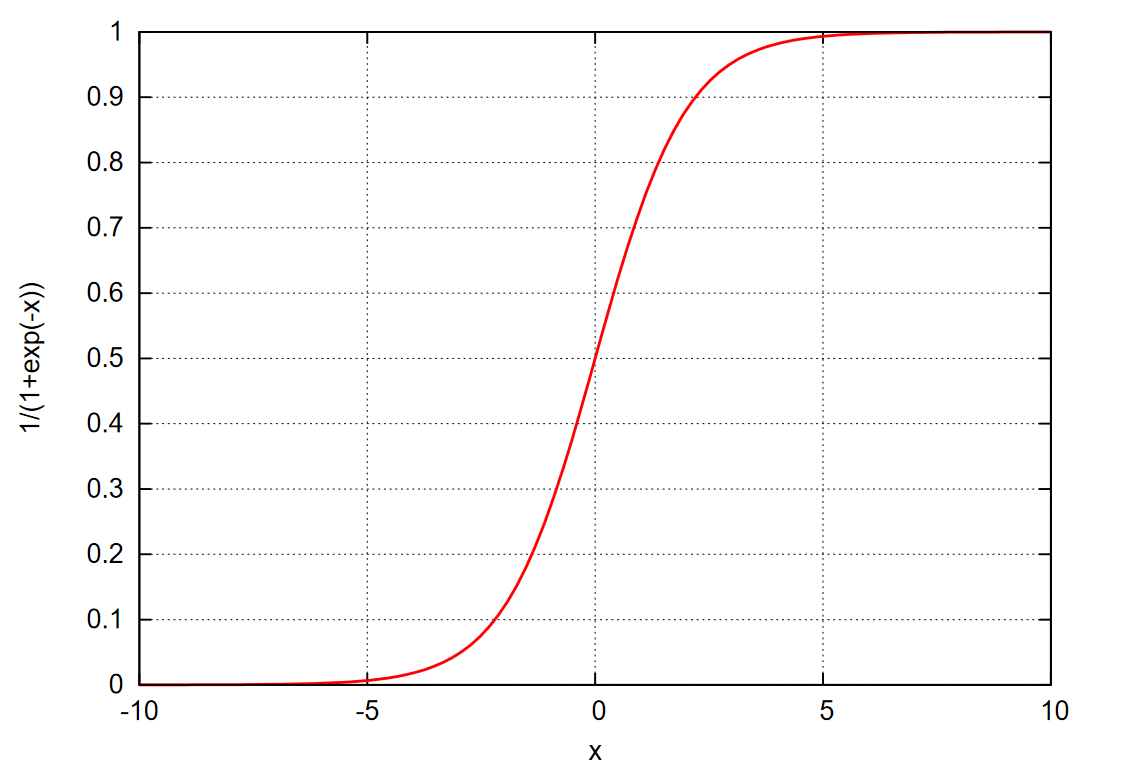
\includegraphics[scale=0.2]{images/sigmoid.png}
    \caption{Sigmoid activation function.}
    \label{fig:sigmoid}
\end{figure}

\textbf{Remark:} this function is derivable and can be plugged into the deep network architecture. \newline

\textbf{Remark:} a problem of this function is that the gradient is almost zero on the left and on the right of its domain. This result in the problem of vanishing gradient. \newline

\section{Output layer}
The deep network architecture can be adopted for many kinds of machine learning problems. \newline

\subsection{Binary classification}
In the case of binary classification we use a single output neuron $o(\pmb{x})$. The sigmoid activation (which allows us to get values between 0 and 1) function becomes:
$$f(\pmb{x}) = \sigma(o(\pmb{x})) = \frac{1}{1+\text{exp}(-o(\pmb{x}))}$$
Then we put a decision threshold at $0.5$.
$$y^* = \text{sign}(f(\pmb{x}) - 0.5)$$

\subsection{Multiclass classification}
In the case of multiclass classification we use one output neuron per class (called \textit{logits} layer):
$$[o_1(\pmb{x}), \hdots, o_c(\pmb{x})]$$
We adopt an activation function which ensures that each output neuron outputs a value between zero and one and that the output of the neurons sum to one. Basically, they represent a probability distribution among the possible classes. The way to do that is to use an activation function:

\begin{equation}
    f_i(x) = \frac{\text{exp}(o_i(\pmb{x}))}{\sum_{j=1}^c \text{exp} (o_j(\pmb{x}))}
\end{equation}

\textbf{Remark:} This is an activation function which is not computed independently for each neuron. It is a layer wise activation function (it requires a normalization step). \newline

\textbf{Remark:} The exponential makes the terms non-negative. Moreover, the normalization ensures that results are between 0 and 1. \newline

The decision is the highest scoring class:
\begin{equation}
    y^* = \text{argmax}_{i \in [1,c]} f_i(\pmb{x})
\end{equation}

\subsection{Regression}
Typically, in the regression case, we take the output of the last layer as it is, using the identity as activation function. \\
We use one output neuron $o(\pmb{x})$. The activation function is linear, \textbf{we delegate to the previous hidden layers the non-linearity of the prediction}. Overall, the decision is the value of output neuron:
\begin{equation}
    f(\pmb{x}) = o(\pmb{x})
\end{equation}

\textbf{Remark:} we do not constraint the values to be in a certain range.

\section{Representational power of MLP}
The purpose of this section is to reason about the representational power of multi-layer perceptrons.
\begin{itemize}
    \item \textbf{boolean functions} Any boolean function can be represented by some network with two layers of units. Indeed, each boolean formula can be written in DNF or CNF form (Figure \ref{fig:brutto_deep_boolean_fun}). For example we can represent a boolean formula expressed in CNF with one neuron for each clause (OR gate), with negative weights for negated literals and one neuron at the top (AND gate). The problem is that these representations can need an exponentially big number of terms. Some functions require an exponential number of gates (e.g. parity function). On the other hand, we can express these functions with linear number of gates with a deep network (e.g. combination of XOR gates).
    
    \item \textbf{continuous functions} Every bounded continuous function can be approximated with arbitrary small error by a network with two layers of units (sigmoid hidden activation, linear output activation).
    
    \item \textbf{arbitrary functions} any function can be approximated to arbitrary accuracy by a network with three layers of units (sigmoid hidden activation, linear output activation).
\end{itemize}

At the end of the day we theoretically need few layers in a deep neural network. However if we adopt few layers, the weights become very difficult to learn. Moreover, we would get an exponentially big number of nodes in each of the layers. In practice, we prefer deep structures rather than shallow networks with exponential number of nodes.

\begin{figure}
    \centering
    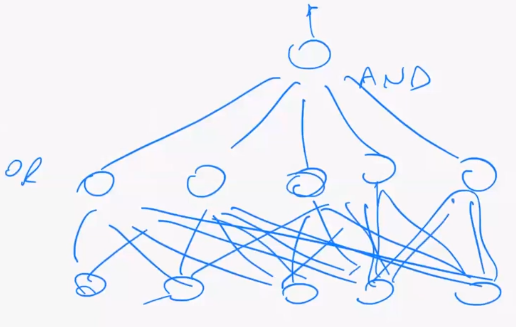
\includegraphics[scale=0.5]{images/brutto_deep_boolean_fun.png}
    \caption{Any boolean function can be represented by some network with two layers of units.}
    \label{fig:brutto_deep_boolean_fun}
\end{figure}

\section{Training MLP}
Similarly to other machine learning models we need to define a loss function and apply gradient based minimization. Some common choices for loss functions are the followings:
\begin{itemize}
    \item \textbf{Cross entropy} for binary classification ($y \in \{0,1\}$)
    \begin{equation}
        \ell(y,f(\pmb{x})) = -(y \log{f(\pmb{x})} + (1-y)\log{(1-f(\pmb{x}))})
    \end{equation}
    Note that the formula compares the expected output with the actual output of the network. If $y=1$ then we take into account the term $\log{f(\pmb{x})}$ otherwise if $y=0$ we take into account the term $\log{(1-f(\pmb{x}))}$. In some ways, the cross entropy tells us the confidence of the given prediction. There is a minus in the front because the higher the value the better the confidence is (secondo me è sbagliata questa frase). We can extend cross entropy also to the case of multiclass classification as explained in the following point.
    
    \item \textbf{Cross entropy} for multiclass classification ($y \in [1,c]$):
    \begin{equation}
        \ell(y, f(\pmb{x})) = -\log{f_y(\pmb{x})}
    \end{equation}
    The minus is to express the cross entropy as an error function instead of a scoring function.
    
    \item \textbf{Mean squared error} for regression:
    \begin{equation}
        \ell(y, f(\pmb{x})) = (y-f(\pmb{x}))^2
    \end{equation}
\end{itemize}
\textbf{Remark:} minimizing cross entropy corresponds to maximizing likelihood. \newline

So, in order to train the neural neural network we identify a proper training error for example $(x,y)$ (e.g. regression):
\begin{equation}
    E(W) = \frac{1}{2} (y - f(x))^2
\end{equation}
and use stochastic gradient descent. Given a learning rate $\nabla$, the gradient update is:
\begin{equation}
    w_{lj} = w_{lj} - \eta \frac{\partial E(W)}{\partial w_{lj}}
\end{equation}
We represent a generic weight in the network with $w_{lj}$ representing the weight of the edge which connects node $j$ of one layer with node $l$ of the following layer (Figure \ref{fig:MLP_stochastic_gradient_descent_brutto}).

\begin{figure}
    \centering
    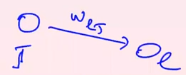
\includegraphics{images/MLP_stochastic_gradient_descent_brutto.png}
    \caption{$w_{lj} = w_{lj} - \eta \frac{\partial E(W)}{\partial w_{lj}}$}
    \label{fig:MLP_stochastic_gradient_descent_brutto}
\end{figure}

The difficult thing is to compute the partial derivative because the weights could be really far from the output layer where we actually compute the error. The solution of this problem is faced with \textit{backpropagation}. The idea is to use the chain rule for derivation. Each weight of the network is updated according to the error computed at the output layer. The notation used in the following formula refers to Figure \ref{fig:backpropagation}.

\begin{equation}
    \frac{\partial E(W)}{\partial w_{li}} = \frac{\partial E(W)}{\partial a_l} \frac{\partial a_l}{w_{lj}} = \delta_l \phi_j
    \label{eq:backpropagation}
\end{equation}

\begin{figure}
    \centering
    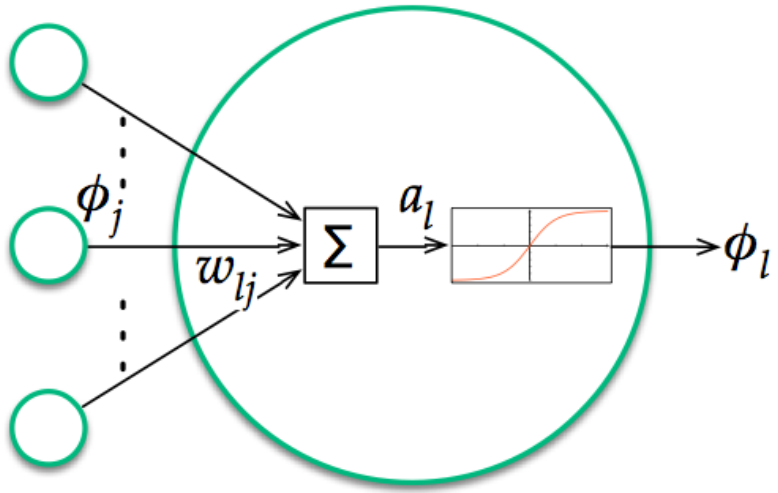
\includegraphics[width=0.5\textwidth]{images/backpropagation.png}
    \caption{The idea of backpropagation is to use the chain rule for derivation.}
    \label{fig:backpropagation}
\end{figure}

\textbf{Remark:} the big circle in Figure \ref{fig:backpropagation} is the node $l$ and $\phi_l$ is the output of node $l$. \newline

Looking inside node $l$ we find the weighted sum of the inputs of the node including $\phi_j w_{lj}$. The result of the summation $a_l$ is the input of an arbitrary activation function. The output of node $l$ is $\phi_l$.\\
In Equation \ref{eq:backpropagation} the aim is to compute the derivative of the error with respect to $w_{ij}$. According to the chain rule this is equale to $\frac{\partial E(W)}{\partial a_l} \frac{\partial a_l}{w_{lj}}$. $a_l$ is the sum of each input of the layer times its weight. As a result the derivative with respect to the weight $w_{lj}$ is the input $\phi_j$. \\
We represent the fraction $\frac{\partial E(W)}{\partial a_i}$ with $\delta_l$. The computation of $\delta_l$ is different if $l$ is a hidden neuron or an output neuron. In what follows, we examine both these cases:
\begin{itemize}
    \item \textbf{Output units}
    Delta is easy to compute on output units. E.g. for regression with linear outputs:
    $$\delta_o = \frac{\partial E(W)}{\partial a_0} = \frac{\partial \frac{1}{2} (y-f(x))^2}{\partial a_0}$$
    Actually $f(x)$ is the result of the application of the non linearity on $a_o$. However, as we said above, in regression we typically do not apply non-linearity at the output layer. As a consequence in this case $f(x)=a_o$.
    $$\delta_o = \frac{\partial \frac{1}{2} (y-a_o)^2}{\partial a_0} = -(y-a_0)$$
    This value allows us to compute the derivative of the error for the weights of the last layer.
    $$\frac{\partial E(W)}{\partial w_{oj}} = \delta_o \phi_j$$
    
    \item \textbf{Hidden units} here we consider the contribution to error through all outer connections (sigmoid activation). Here $l$ is not an output node but an internal node. The error $E$ is computed at the very top of the graph illustrated in Figure \ref{fig.training_mld_hidden_units}, in the red node. As a result we have to backpropagate this error through the network structure.\\
    The derivative of the error $\frac{\partial E(W)}{\partial a_l}$ is decomposed into the derivative of the error with respect to each of the nodes which follow $l$.
    $$\delta_l = \frac{\partial E(W)}{\partial a_l} = \sum_{k \in \text{ch}[l]} \frac{\partial E(W)}{\partial a_k} \frac{\partial a_k}{\partial a_l}$$
    Intuitively we are calculating the contribution of $l$ to the error at the end of the structure.\\
    Now we notice that the $\frac{\partial E(W)}{\partial a_k}$ is actually $\delta_k$ (recursion). Moreover, remember that the output of $l$ is represented with $\phi_l$.
    $$\delta_l = \sum_{k \in \text{ch}[l]} \frac{\partial E(W)}{\partial a_k} \frac{\partial a_k}{\partial a_l} = \sum_{k \in \text{ch}[l]} \delta_k \frac{\partial a_k}{\partial \phi_l} \frac{\partial \phi_l}{\partial a_l}$$
    We assign weight $w_{kl}$ to the edge $(k,l)$. As a consequence $\frac{\partial a_k}{\partial \phi_l} = w_{kl}$. Moreover, $\frac{\partial \phi_l}{\partial a_l}$ is essentially the derivation of the activation function with respect to its input.
    $$\delta_l = \sum_{k \in \text{ch}[l]} \delta_k \frac{\partial a_k}{\partial \phi_l} \frac{\partial \phi_l}{\partial a_l} = \sum_{k \in \text{ch}[l]} \delta_k w_{kl} \frac{\partial \sigma(a_l)}{\partial a_l}$$
    In this case we take into account the sigmoid activation function.
    $$\delta_l = \sum_{k \in \text{ch}[l]} \delta_k w_{kl} \frac{\partial \sigma(a_l)}{\partial a_l} = \sum_{k \in \text{ch}[l]} \delta_k w_{kl} \sigma(a_l) (1 - \sigma(a_l))$$
\end{itemize}

\begin{figure}
    \centering
    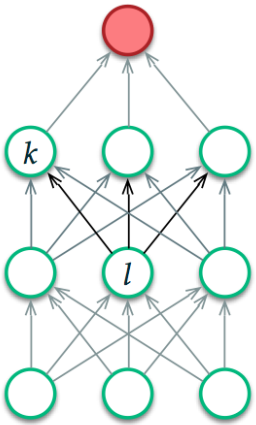
\includegraphics[scale=0.7]{images/mlp_learning_hidden_layer.png}
    \caption{Consider contribution to error through all outer connection.}
    \label{fig.training_mld_hidden_units}
\end{figure}

In deep neural network, the neural architectures are really seen as combinations of modules (Figure \ref{fig:deep_architectures:modular structure}). Each of these modules has an interface to interact with the outside. The aim is to combine modules in order to construct a deep architecture. In Figure \ref{fig:deep_architectures:modular structure} we understand how this architecture looks like and how it is updated.

\begin{itemize}
    \item We have a first layer $F_1(x, W_1)$ which takes input $x$ and weight matrix $W_1$ and computes $\phi_1$.
    
    \item The second layer $F_2(\phi_1, W_2)$ takes as input $\phi_1$ and weight matrix $W_2$ and computes the new representation of the input $\phi_2$.
    
    \item In the output layer we apply a loss function $\text{Loss}(\phi_3, y)$. With this module we compute the error for having predicted a certain value instead of $y$. With this error value we can compute $\frac{\partial E}{\partial \sigma_3}$.
    
    \item At this point, the $\frac{\partial E}{\partial W_j}$ can be decomposed as:
    $$\frac{\partial E}{\partial W_j} = \frac{\partial E}{\partial \phi_j} \frac{\partial \phi_j}{\partial W_j} = \frac{\partial E}{\partial \phi_j} \frac{\partial F_j(\phi_{j-1}, W_j)}{\partial W_j}$$
    At the very end of the chain the output layer produces $\frac{\partial E}{\partial \phi_j}$. However, each arbitrary layer needs this information from the following layer. Each layer should be able to propagate this information to the layer below. So, each layer can compute $\frac{\partial E}{\partial \phi_{j-1}}$. For example layer three in Figure \ref{fig:deep_architectures:modular structure} is able to compute $\frac{\partial E}{\partial \phi_{2}}$.
    $$\frac{\partial E}{\partial \phi_{j-1}} = \frac{\partial E}{\partial \phi_{j}} \frac{\partial \phi_j}{\partial \phi_{j-1}} = \frac{\partial E}{\partial \phi_{j}} \frac{\partial F_j(\phi_{j-1}, W_j)}{\partial \phi_{j-1}}$$
    
    \item Each module should be able to compute the derivative of its output with respect to its weights ($\frac{\partial F_j(\phi_{j-1}, W_j)}{\partial W_j}$). Moreover, each module should be able to compute the derivative of its output with respect to its inputs ($\frac{\partial F_j(\phi_{j-1}, W_j)}{\partial \phi_{j-1}}$). The former is used by the module to update its own weights and the latter is used by the module to backpropagate the error. This allows to following layers down in the hierarchy to update their own weights.
\end{itemize}

Overall, this is a modular architecture: we do not care about what $F_j$ does internally. \newline

\begin{figure}
    \centering
    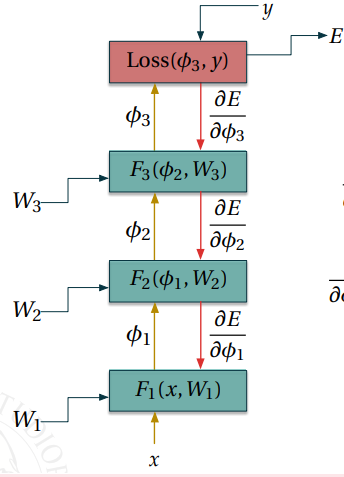
\includegraphics[width=0.6\textwidth]{images/deep_modules.png}
    \caption{In deep neural network, the neural architectures are really seen as combinations of modules.}
    \label{fig:deep_architectures:modular structure}
\end{figure}

At the end of the day with backpropagation we perform gradient descent. Hence, backpropagation is only guaranteed to converge to a local minimum. Moreover, the error surface of a multilayer neural network can contain several minima. The literature proposes heuristic attempts to address the problem (the problem in question is that backpropagation is only guaranteed to converge to a local minimum):
\begin{itemize}
    \item use stochastic instead of true gradient descent
    \item train multiple networks with different random weights and average or choose best
    \item random restart of the weights
    \item many more...
\end{itemize}

\textbf{Remark:} training kernel machines requires solving quadratic optimization problems. As a result, finding the global optimum is guaranteed (convex problem). On the other hand deep networks are more expressive in principle, but harder to train.

\subsection{Stopping criterion and generalization}
Commonly the validation set is used to choose the best configuration of the hyperparameters. In deep learning we can still use the validation set to configure the hyperparameters. However, in deep learning we can use the validation set to choose the training termination condition. Actually, overtraining the network increases possibility of overfitting training data (we could progressively fit noise penalizing generalization). Neural network models are really expressive, which means that they are complex, which means that they are prone to overfitting. In particular, overfitting occurs at later iterations, when increasingly complex surfaces are being generated. Note that at the beginning, the network is initialized with small random weights and so the decision surface is very simple. Overall, the aim is to stop learning before starting learning the noise. To do this, we use a separate validation set to estimate performance of the network and choose when to stop training. As we can seen in Figure \ref{fig:deep_training_test_valudation}, the error on the validation set at some point (when the model begins to overfit) starts to increase. In practice, we keep track of the validation error; we periodically save the best weights seen in the validation set; we stop learning when we notice that the validation error starts to increase. Probably in the case of Figure \ref{fig:deep_training_test_valudation} we keep learning until epoch 9 and then we keep the weights learned at epoch 5.\\ This technique is referred to as \textit{early stopping}. \newline

\textbf{Remark:} in backpropagation we typically do not take into account all the examples of the training set in order to compute the error in the output layer and update the weights. Typically, we perform as an alternative, mini-batch gradient descent.

\begin{figure}
    \centering
    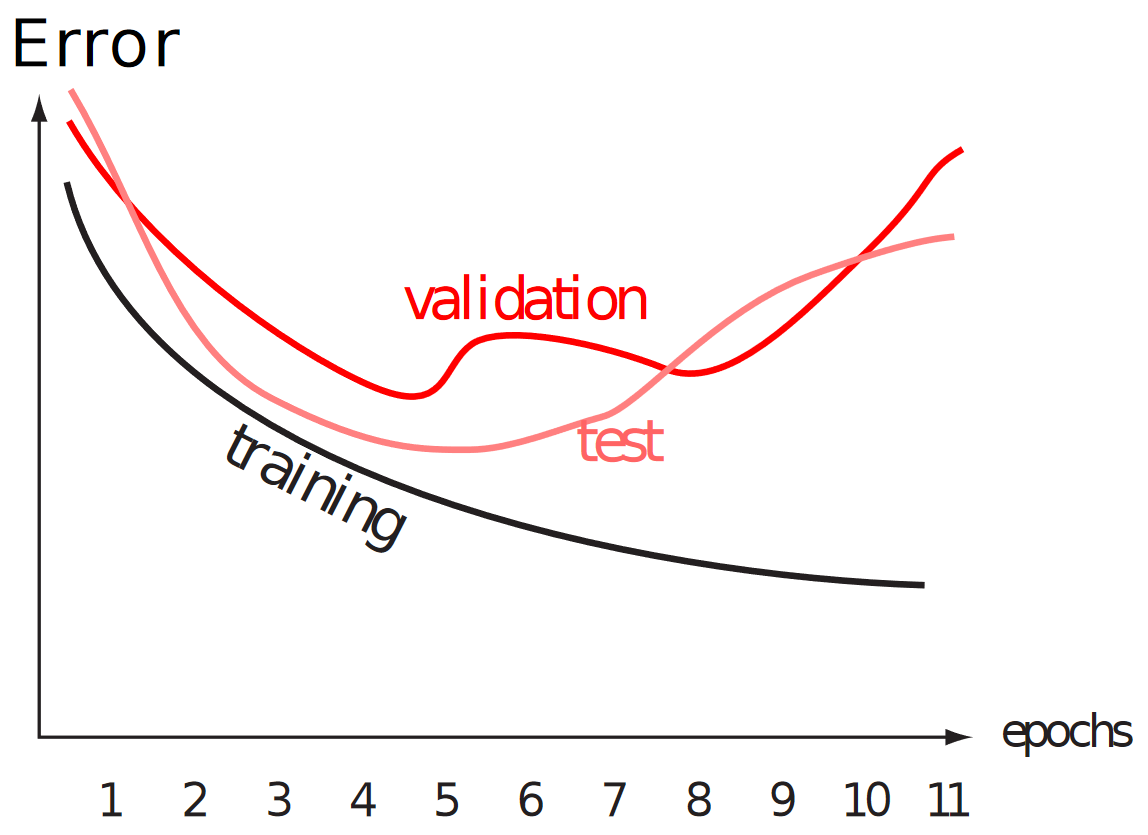
\includegraphics[width=0.5\textwidth]{images/deep_training_test_valudation.png}
    \caption{Training error, validation error, test error in deep learning.}
    \label{fig:deep_training_test_valudation}
\end{figure}

\subsection{The problem of vanishing gradient}
Training a neural network is not a convex problem, hence there are more things that might go wrong than SVMs. The problem of vanishing gradient together with the lack of training data and the limited amount of computation power are perhaps the most common reasons why deep learning has become a hot research topic only in the last ten years. As we discussed above, the main idea of backpropagation is that the error gradient (somehow a signal) is backpropagated through layers. At each step gradient is multiplied by derivative of sigmoid. A problem of the sigmoid function is that it saturates for small values and large values of its input. The gradient is informative where the sigmoid behaves almost linearly, but it is zero or close to zero in the saturation areas. At some point of the training process we might start propagating values of the gradient which are almost zero. This problem is known as \textit{vanishing gradient}: the gradient vanishes in lower layers. \newline

In the following we present few simple suggestions:
\begin{itemize}
    \item Do not initialize weights to zero, but to small random values around zero. In this way we somehow inject diversity inside the network avoiding that all the neurons learn in the same way.
    
    \item It is possible to have to deal with datasets characterized by inputs with very different range. Some numbers between 0 and 100, some other numbers between -10000 and 100000 for instance. This results in a high probability to fall in the saturation area of the activation functions or in very high (or very small) values of the weights to balance the structure. A valid trick is to standardize inputs to avoid saturating hidden units:
    $$x' = \frac{(x - \mu_x)}{\sigma_x}$$
    In order to standardize an input, for each possible feature, we have to subtract the mean and divide by the standard deviation. In this way each feature is 0 mean and 1 standard deviation.
    
    
    \item Randomly shuffle training examples before each training epoch. In this way we ensure that at each epoch examples are presented in a different order.
\end{itemize}

Perhaps, one of the main reasons why this architecture started to be trainable is the realization of the community that the saturated areas of the sigmoid were the main caveats for which backpropagation did not work properly. As a result the literature came out with an alternative (still non linear) activation function. This last is called \textit{ReLU} (rectified linear unit):
\begin{equation}
    f(x) = \text{max}(0, \pmb{w}^T \pmb{x})
\end{equation}

\textbf{Remark:} Essentially, the ReLU returns the maximum between zero and the input of the activation function ($\pmb{w}^T \pmb{x}$) where $\pmb{x}$ is the input of the neuron. \newline

\textbf{Remark:} somehow this function is similar to the hinge loss. \newline

As we can see in Figure \ref{fig:relu} this function brings everything to zero if the input is negative, while on the right is linear. The function saturates only on the left. As a consequence we have more chance to avoid vanishing gradient problem. \newline

To sum up:
\begin{itemize}
    \item Linearity is nice for learning
    \item Saturation (as in sigmoid) is bad for learning (gradient vanishes implies no weight update)
    \item Neuron employing rectifier activation called rectified linear unit (ReLU)
\end{itemize}

\begin{figure}
    \centering
    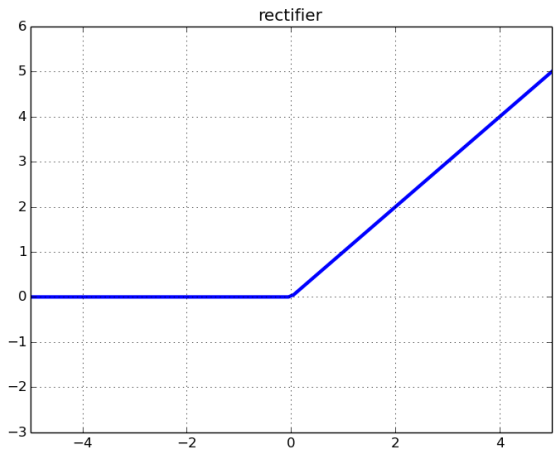
\includegraphics[scale=0.5]{images/relu.png}
    \caption{Rectified Linear Unit (ReLU)}
    \label{fig:relu}
\end{figure}

Another trick of the trade to face the problems related to the training of a deep neural network is regularization. As discussed above in the text, the aim of regularization theory is to minimize both model complexity and training error. So the objective function ($J(W)$) is composed by two terms: the error ($E(W)$) on the training set and the complexity of the model ($\lambda ||W||_2$) with the tradeoff parameter $\lambda$:
$$J(W) = E(W)+\lambda ||W||_2$$

For the sake of simplicity, in Figure \ref{fig:deep_regularization} we assume to have two weights ($W_1$ and $W_2$). The Euclidean norm (or 2-norm) of the weights is something that is minimal at zero and grows in circles. This means that points on the same circle have the same norm, they are indistinguishable with respect to the minimization of the regularization term $||W||_2$. Then, suppose the error function is an ellipsoid which is minimal in the center. Depending on the value of $\lambda$ we decide a tradeoff between the two objectives to minimize. With this procedure we end up choosing a point where the regularization circle touches the error ellipsoid. \newline

In essence \textit{2-norm regularization} penalizes weights by Euclidean norm. Weights with less influence on error get smaller values. \newline

\begin{figure}
    \centering
    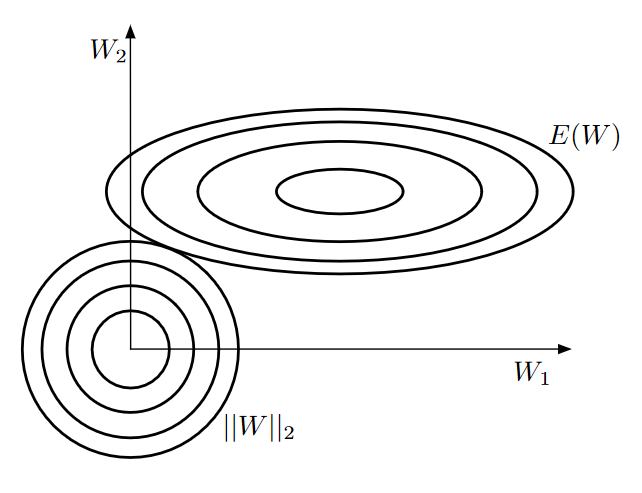
\includegraphics[scale=0.5]{images/deepRegularization.png}
    \caption{Regularization allows us to penalize weights by Euclidean norm: weights with less influence on error get smaller values.}
    \label{fig:deep_regularization}
\end{figure}

There is an alternative form of regularization that can be used which is \textit{1-norm regularization} (Figure \ref{fig::1NormRegularization}):
$$J(W) = E(W) + \lambda |W|$$
In this case the regularization penalizes weights by sum of absolute values ($|w| = \sum_i |w_i|$). In this case the ball around zero is no more a circle but something like a square. Of course, points on the same square have the same norm. This encourages less relevant weights to be exactly zero (sparsity inducing norm). Indeed, in the previous case the circle touches the ellipsoid at a random point, on the other hand in this case the square is more likely to touch the ellipsoid at the vertices. Note that if we touch the square at a vertex some of the weights are zero. This is called \textit{sparsifying norm}: a norm which encourages sparse solutions. This kind of regularization can be useful when we want to minimize the number of weights in the solution for instance for interpretability or for feature selection. \newline

\begin{figure}
    \centering
    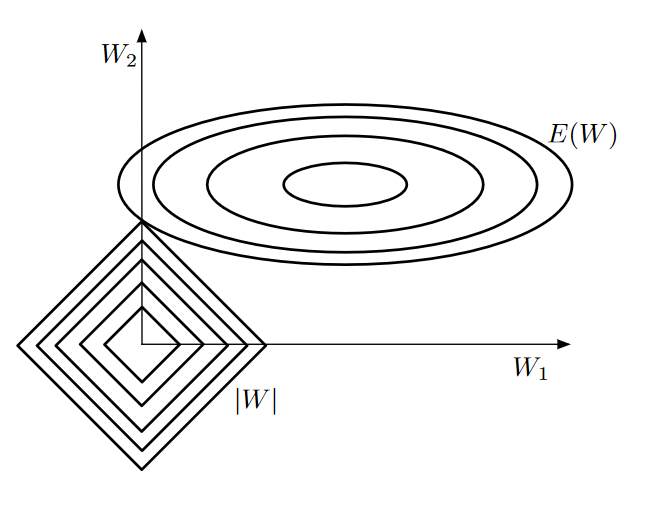
\includegraphics[scale=0.5]{images/1NormRegularization.png}
    \caption{Regularization penalizes weights by sum of absolute values. This encourages less relevant weights to be exactly zero (sparsity inducing norm).}
    \label{fig::1NormRegularization}
\end{figure}

Another trick of the trade to face the problems related to the training of a deep neural network is initialization. First of all it is important to randomly initialize weights. In this way we break symmetries between neurons. Indeed, if we initialize all weights to zero they might all learn the same thing becoming redundant. This would reduce the overall expressiveness of the network. In order to carefully set the initialization range to preserve forward and backward variance we use the following formula:
$$W_{ij} \sim U(- \frac{\sqrt{6}}{\sqrt{n+m}}, \frac{\sqrt{6}}{\sqrt{n+m}})$$
where $n$ and $m$ are number of inputs and outputs. Overall, the aim is to ensure sparse initialization: enforce a fraction of weights to be non-zero (this encourages diversity between neurons). \newline

Another trick of the trade to face the problems related to the training of a deep neural network is minibatch gradient descent. Batch gradient descent updates parameters after seeing all examples (of the training set). This procedure is too slow for large datasets. On the other hand, full stochastic gradient descent updates parameters after seeing each example. In a large network, the error that we compute for a single example can be quite different from the error that is averaged over many examples. Overall, the objective would be too different from the true one. A valid solution is an intermediate technique between batch and fully stochastic gradient descent. \textit{Minibatch} gradient descent divides the training set into minibatches and updates parameters after seeing a minibatch of $m$ examples. The proper value of $m$ depends on many factor, e.g. size of GPU memory. Indeed, our architectural consideration is that we do not want a minibatch too large which does not fit the GPU memory. \newline

Another trick of the trade to face the problems related to the training of a deep neural network is a proper configuration of the learning rate. With this aim an popular approach is the usage of the \textit{momentum} concept. The idea is to update the weights not only depending on the current direction of the gradient but also partially according to the directions of the previous iterations. The tradeoff is regulated by a coefficient $\alpha$ called momentum.
$$v_{ji} = \alpha v_{ji} - \eta \frac{\partial E(W)}{\partial w_lj}$$
$$\pmb{w}_{ji} = w_{ji} + v_{ji}$$
where $0 \leq \alpha < 1$.
The adoption of the momentum tends to keep the updating of the weights in the same direction. Think of a ball rolling on an error surface. The possible effects could be:
\begin{itemize}
    \item roll through small local minima without stopping
    
    \item traverse flat surfaces instead of stopping there
    
    \item increase step size of search in regions of constant gradient
\end{itemize}

Another trick of the trade to face the problems related to the training of a deep neural network is the usage an adaptive (decreasing) learning rate. The idea is to use larger learning rate at the beginning (when we are far from the optimum) for faster convergence towards attraction basin. Then, smaller learning rate at the end to avoid oscillation close to the minimum. Indeed with too big oscillation, we could miss the optimum.

$$\eta_t =
\begin{cases}
    (1-\frac{t}{\tau})\eta_0 + \frac{t}{\tau} \eta_{\tau} &\text{if $t<\tau$}\\
    \eta_\tau &\text{otherwise}
\end{cases}$$

In the formula, after a certain number of iterations $\tau$, $\eta_t$ becomes $\eta_\tau$. Before, the learning rate is a combination of the two. While the procedure progressively reaches the optimum, the learning rate progressively goes from $\eta_0$ to $\eta_\tau$. \newline

Another trick of the trade to face the problems related to the training of a deep neural network is related to the \textit{Adagrad} approach.

$$r_{ji} = r_{ji} + (\frac{\partial E(W)}{\partial w_{lj}})^2$$
$$\pmb{w}_{ji} = w_{ji} - \frac{\eta}{\sqrt{r_{ji}}} \frac{\partial E(W)}{\partial w_{lj}}$$

Using momentum we vary the learning rate only with respect to time, but the learning rate value is the same for all the directions. In high-dimensional problems, the behaviour of the function can be very different in each direction. From this, we understand that using the same learning rate for all directions is clearly suboptimal. The idea of the adagrad approach is to develop an adaptive gradient such that:
\begin{itemize}
    \item Reduce learning rate in steep directions
    \item Increase learning rate in gentler directions
\end{itemize}

Intuitively $r_{ji}$ accumulates the square of the partial derivatives for a certain dimension. This means that if a certain dimension has a high value of the derivative for a lot of iterations, the function is steep along that dimension. So, the learning rate is divided by this size of the gradient ($\frac{\eta}{\sqrt{r_{ji}}}$). (The square root is needed to scale the value in the order of the weights, avoiding the square term).\\
Overall, adagrad is actually a good solution to speed up convergence in high dimensional spaces. However, we can highlight a problem of this procedure:
\begin{itemize}
    \item The square gradient is accumulated over all iterations. This could lead to non-local decisions. This means that the reduction of the learning rate could become too large at some point. For non-convex problems, learning rate reduction can be excessive/premature.
\end{itemize}
To solve this problem, the literature propose an alternative called \textit{RMSProp}.

$$r_{ji} = \rho r_{ji} + (1 - \rho) (\frac{\partial E(W)}{\partial w_{ij}})^2$$
$$\pmb{w}_{ji} = w_{ji} - \frac{\eta}{\sqrt{r_{ji}}} \frac{\partial E(W)}{\partial w_{lj}}$$
The most relevant difference with respect to the previous approach is that we calculate a linear combination ($\rho r_{ji} + (1 - \rho) (\frac{\partial E(W)}{\partial w_{ij}})^2$) of the current value and the new squared gradient. In this way, we obtain an exponentially decaying accumulation of squared gradient ($0<\rho<1$). The squared gradient is exponentially decaying with respect to how far we are from the current position. So, old values of the gradient do not count anymore in order to decide whether to slow down or not. In this way the update of the learning rate becomes more local. Doing this, RMSProp avoids the premature reduction of Adagrad and the respective slowing down. Poi sulle slide c'è scritto Adgrad-like behaviour when reaching convex bowl, ma non so bene cosa si intenda. \newline

The update rule for neural networks which is the defacto standard is a variant of the methods we have discussed, which is called ADAM. \newline

Another trick of the trade to face the problems related to the training of a deep neural network is \textit{batch normalization}. This concept is related to the so called \textit{covariate shift problem}. Covariate shift problem is when the input distribution to your model changes over time and the model does not adapt to the change. The fact that the input distribution changes over time is problematic. Indeed, when we train a model we typically assume that examples are independent and identically distributed (i.i.d.). If we consider examples whose distribution changes over time, they are no more identically distributed. The learning model should adapt continuously to the change of the data. In (very) deep networks, internal covariate shift takes place among layers when they get updated by backpropagation. Basically, the update of a layer refers to a representation of the data which is old with respect to the current collection of examples. This leads to a slower convergence: we need to keep adjusting the weights according to the changes in the network. \newline

\textbf{Remark:} according to the web the term covariate refers to an independent variable that can influence the outcome of a given statistical trial, but which is not of direct interest. Other definitions more related to the topic at hand are welcome. \newline

Batch normalization is a solution proposed by the literature to solve this problem. The idea is to normalize each node activation (input to activation function) by its batch statistics in order to keep it always in the same range. This prevents the covariate shift since for each layer the activation to the activation function stays in the same range.

$$\hat{x_i} = \frac{x_i - \mu_B}{\sigma_B}$$

where:
\begin{itemize}
    \item $x$ is the activation of an arbitrary node in an arbitrary layer
    
    \item $\mathcal{B} = \{x_1, \hdots, x_m\}$, is a batch of values for that activation
    
    \item $\mu_\beta$, $\sigma_B^2$ are batch mean and variance (for each neuron)
\end{itemize}

Keeping the activation always in the same range is in contrast with respect to the aim of learning a suitable configuration of the deep neural network. Perhaps, we could end up to concentrate the activation in the same range too much. To avoid this we combine the normalization with scale and shift parameters ($\gamma$, $\beta$).
$$y_i = \gamma \hat{x}_i + \beta$$
In this manner, we scale and shift each activation with adjustable parameters. In this way the standardized activation is adjusted before being processed by the activation function. \newline

\textbf{Remark:} the scale $\gamma$ and shift $\beta$ coefficients become part of the network parameters and they have to be learnt. \newline

Some advantages of batch normalization are:
\begin{itemize}
    \item More robustness of parameter initialization
    
    \item Allows for faster learning rates without divergence
    
    \item Keeps activations in non-saturated region even for saturating activation functions. In this sense, in some cases, we could use the sigmoid activation function if we adopt batch normalization
    
    \item Regularizes the model
\end{itemize}

Another trick of the trade to face the problems related to the training of a deep neural network is \textit{layerwise pre-training}. Modern solution for pre-training are:
\begin{itemize}
    \item Supervised pre-training: layerwise training with actual labels
    
    \item Transfer learning: train network on similar task, discard last layers and retrain on target task
    
    \item Multi-level supervision: auxiliary output nodes at intermediate layers to speed up learning
\end{itemize}
Nota: non ho capito benissimo questi punti. Non vengono spiegati o approfonditi molto bene ma non credo siano importanti ai fini dell'esame.

\section{Many different architectures}
At this point we overview the main deep neural network architectures as an alternative of the multilayer perceptron. In this context, the literature proposes many different architectures:

\begin{itemize}
    \item \textit{convolutional networks} for exploiting local correlations (e.g. for images).
    
    \item \textit{recurrent} and \textit{recursive} networks for collective predictions (e.g. sequential labelling). This model are useful for inputs which are not vectors but sequences (sequential data) or other structures (e.g. graph neural network).
    
    \item \textit{deep Boltzmann machines} as probabilistic generative models (can also generate new instances of a certain class). Another example of deep generative model are variatonal autoencoders. These kind of generative models do not need to model directly the probabilistic relationships between single variables in terms of conditional probability distributions as we studied in the case of Bayesian networks.
    
    \item \textit{generative adversarial networks} to generate new instances as a game between discriminator and generator. In general, the aim is to learn a model which is able to generate objects which are similar to the ones which are seen in input.
\end{itemize}

\subsection{Autoencoder}
The \textit{autoencoder} is a deep neural architecure whose purpose is to train shallow network to reproduce input in the output. In other words, the autoencoder is trained to recunstruct its intput. As we can see in Figure \ref{fig:autoencoder} the structure has the same number of inputs and outputs. Moreover, we can notice that there is only one internal layer, called \textit{coding layer}. \\ Once the autoencoder is trained, its purpose is to process $x$ as input and provide $x$ as output. This process can be done with unlabelled examples in a \textit{unsupervised learning} fashion.\\
As an example, one can structure the code layer in such a way that handwritten digits are encoded in the hidden layer with a binary representation. In general, the aim of the autoencoder is to learn to map inputs into a sensible hidden representation (\textit{representation learning}). From this representation it should be possible to reconstruct the original input. As a consequence, the autoencoder is often used to map data in a different dimensional space. Another typical application of autoencoders is to generate data from the representation that has been learned. Autoencoders were also adopted to perform layerwise pre-training (Figure \ref{fig:autoencoder_layerwise1}, Figure \ref{fig:autoencoder_layerwise2}):
\begin{enumerate}
    \item train the autoencoder
    \item discard the output layer
    
    \item freeze hidden layer weights
    
    \item add another hidden layer and another output layer
    
    \item train network to reproduce input
\end{enumerate}
In this way we learn a representation of the input which is more abstract than the first one, but that can still reconstruct the original input. \\ We can use the output of this approach (as deep as we want) in supervised learning task:
\begin{enumerate}
    \item discard autoencoder output layer
    \item add appropriate output layer for supervised task (e.g. one-hot encoding for multiclass classification)
    \item learn output layer weights and refine all internal weights by backpropagation algorithm
\end{enumerate}
Intuitively, the hidden layers of the final network are designed to conserve as much information of the input as possible. \newline

\textbf{Remark:} studying autoencoders we can highlight a crucial difference with respect to kernel machines. With autoencoders the model learns a suitable data representation, on the other hand kernel machines propose an engineered representation $\phi(x)$ which is given and not learnt. In general, in neural network the architecture is engineered while the feature mapping is learnt. \newline

Nowadays, autoencoders are no more used to perform layerwise pre-training.

\begin{figure}
    \centering
    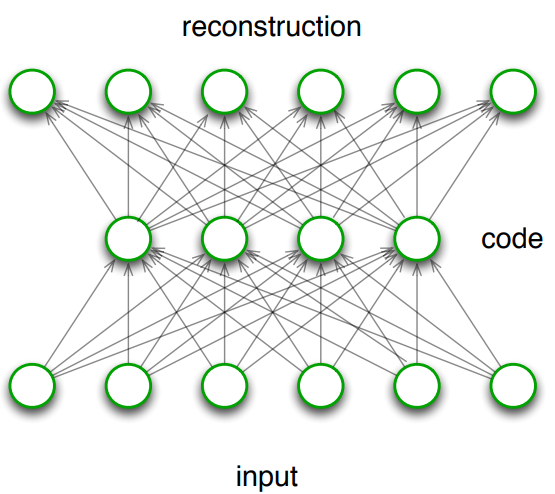
\includegraphics[scale = 0.5]{images/autoencoder.png}
    \caption{Autoencoder}
    \label{fig:autoencoder}
\end{figure}

\begin{figure}
    \centering
    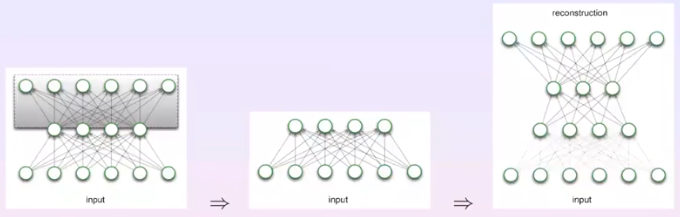
\includegraphics[width=\textwidth]{images/autoencoder_layerwise1.png}
    \caption{Layerwise pre-training with autoencoder 1.}
    \label{fig:autoencoder_layerwise1}
\end{figure}

\begin{figure}
    \centering
    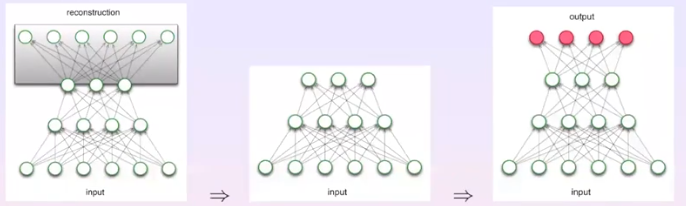
\includegraphics[width=\textwidth]{images/autoencoder_layerwise2.png}
    \caption{Layerwise pre-training with autoencoder 2.}
    \label{fig:autoencoder_layerwise2}
\end{figure}

\subsection{Convolutional network (CNN)}
\textit{Convolutional neural networks} (Figure \ref{fig:cnn}) are a consolidated architecture in the field of image processing and image classification. Images are seen as two dimensional matrices of pixels or as multidimensional objects. For example, we can imagine an image as a structure composed by an additional channel representing image color (we often use a matrix for each channel). CNNs allow to understand correlations among spatially closed pixels. Moreover, convolutional neural network has to implement location invariance (e.g. translation inside the image): if we detect a boat, its position inside the image does not affect the classification output. In order to achieve these purposes CNNs use \textit{convolution filters}. These are matrices of weights which are used to scan the image from the very top down to the end. Each input portion of the image inside the matrix is combined (aggregated) into one value. A convolutional neural network can adopt more than one filter. Every filter produces its own representation for the given image. The purpose of convolution filters is to extract local features. \\ In addition to convolution, CNNs perform also pooling to provide invariance to local variations. Pooling allow us to combine the local prediction in a small area, and this leads to more robustness against translations for example. A common pooling implementation is \textit{max pooling} where we take the maximum value of the matrix in a certain area. The maximum value is used to produce a new smaller representation of the matrix. \\ Overall, convolution filters and pooling are the two main components of a CNN such that:
\begin{itemize}
    \item filters should learn to identify patterns inside the input image
    
    \item the pooling process tries to understand if in the given area it has been found something 
\end{itemize}

A combination of filters and convolution layers is repeated along the network in order to progressively find higher level patterns. The first layers understand simple patterns like straight lines; subsequently, further layers can combine patterns to construct more complex and higher level patterns. In this way we obtain a hierarchy of filters to compose complex features from simpler ones (e.g. pixels to edges to shapes). All these matrices are learnt in an end to end fashion. \\
At some point the convolutional neural network ends with a multi layer perceptron architecture: all the features are placed in a vector and processed with densely fully connected layers. Finally, at the output level we reach a representation which allows us to perform the (e.g. classification) task.

\begin{figure}
    \centering
    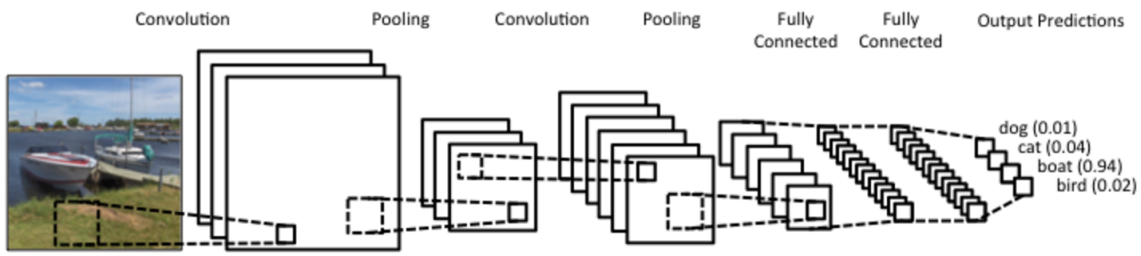
\includegraphics[width=\textwidth]{images/cnn.png}
    \caption{Convolutional neural network.}
    \label{fig:cnn}
\end{figure}

\subsection{Long Short-Term Memory Networks (LSMT)}
Recurrent neural networks allow to make predictions about objects which are not fixed size vectors but for example sequences. We discussed about kernel techniques which are used to process sequences. In this subsection we introduce a template based model which is used to process sequences to obtain representations which are suitable for learning. As illustrated in Figure \ref{fig:lsmt} the architecture is composed by the same unit repeated a number of times equal to the number of inputs. Each unit processes an input obtaining an output which is sent to the following unit. The result is a propagation of information from input to output. Looking inside an unit:

\begin{itemize}
    \item $\sigma$ are parametric layers which end with the sigmoid. The sigmoid function restricts the input in a range between zero and one. We can see this value as a probabilistic value.
    
    \item Somewhere inside the unit products are computed. In Figure \ref{fig:lsmt} they are are represented with a X. These are element wise products.
    
    \item These operations allow to learn a state inside the unit and propagate it along the network.
    
    \item During the multiplications, if the value (I think of the sigmoid) for a certain dimension is zero, we reset that dimension (I think the state associated with that dimension). On the other hand, if the value (I think of the sigmoid) is one we keep that dimension as it is. Then, if the value (I think of the sigmoid) is between zero and one, the dimension is down-weighted.
\end{itemize}

At the end of the day we obtain a recurrent computation with selective memory such that:
\begin{itemize}
    \item a cell state is propagated along the chain
    
    \item a forget gate selectively forgets parts of the cell state. Implicitly we also select which part of the state to remember to go to the next state.
    
    \item an input gate selectively chooses parts of the candidate (i.e. input) for cell update (i.e. update the state, actually, after the multiplication there is a plus operation). In essence, the same concept of the forget gate is applied to the input itself. Indeed, in Figure \ref{fig:lsmt} we can notice a sigma layer which is multiplied with the input. 
    
    \item Finally output gate selectively chooses parts of the cell state for output
\end{itemize}

Inside a cell, the overall state is a combination of the part of the previous state which has been not forgotten (this is represented by the first X inside the second network unit in Figure \ref{fig:lsmt}) and a selected part of the information that we get from the input (this is represented by the plus after the first X in Figure \ref{fig:lsmt}). This combination produces the updated state which is propagated to the next unit. Before being propagated, this state is combined with the output gate (that depends also on the input, look at the arrow from $\sigma$ in the top right of the figure to output in Figure \ref{fig:lsmt}) to decide what parts of the cell state have to be sent as the output of the given unit. Moreover, the output of the current unit will become part of the combination of the local input and the propagated state of the following unit. \\
In Figure \ref{fig:lsmt}, letter $h$ at each unit is the representation at each state that has been learnt. According to the task at hand, we can add (for example) a classification or a regression layer on top of $h$ (basically everything we need to perform the final prediction). \newline

The most relevant thing of this gate architecture is that all the gates are parametric, are learnt. In this way, the network decides what to remember, what to use to update, what to output, at each unit. This kind of architecture is commonly referred to as \textit{long short-term memory} because it adaptively decides what to remember. We can use this structure for example to avoid forgetting a signal which is propagated too long in time. The selective memory can decide what to remember, simplifying the task of remembering something for a long time. In this sense, this architecture works well in sequential prediction tasks.

\begin{figure}
    \centering
    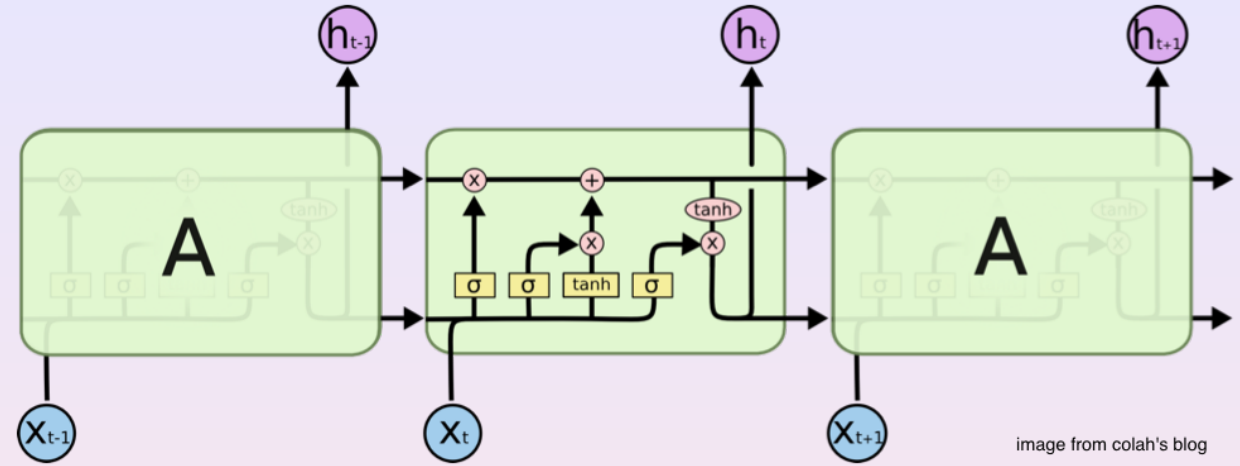
\includegraphics[width=\textwidth]{images/lsmt.png}
    \caption{Long Short-Term Memory Networks (LSMT).}
    \label{fig:lsmt}
\end{figure}

\subsection{Generative Adversarial Networks (GAN)}
Another popular deep architecture is the \textit{generative adversarial network} (Figure \ref{fig:generative_adversarial_network}). The goal of GANs is to generate new objects. The task of generating new data can become extremely complicated when dealing with high dimensions. The architecure is composed by:
\begin{itemize}
    \item a \textit{generator} network which learns to generate items (e.g. images) from random noise. The generator is trained in order to fool the discriminator. Sometimes we refer to the generator as the \textit{forger}.
    
    \item a \textit{discriminator} network which learns to distinguish between real items and generated ones. The discriminator is trained taking as input a dataset of real images (positive examples) and images generated by the generator neural network (negative examples). Sometimes we refer to the generator as the \textit{detective}.
\end{itemize}
The two networks are jointly learnt as in an adversarial game. Along the process no human supervision is needed.

\begin{figure}
    \centering
    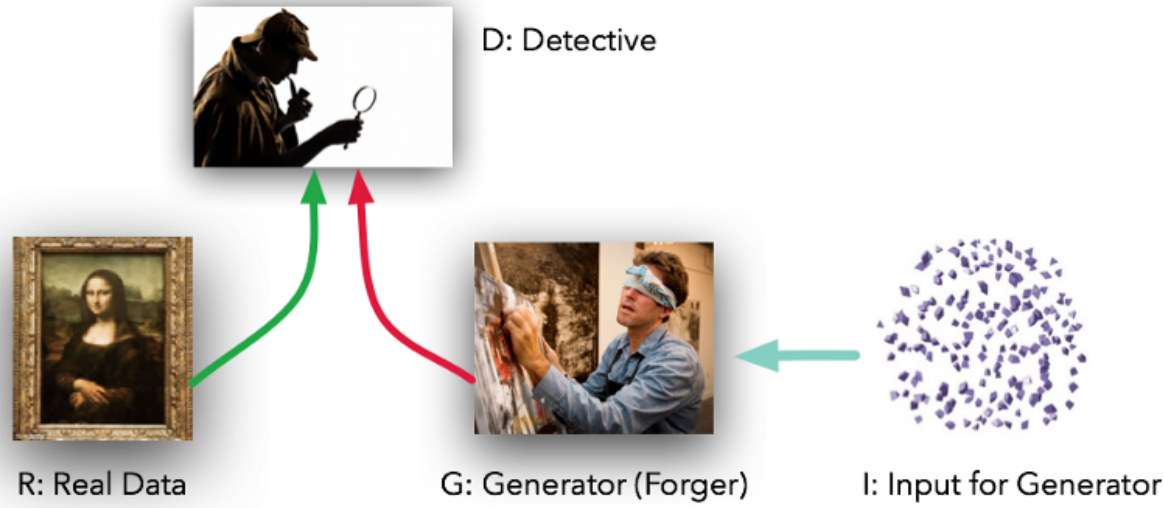
\includegraphics[width=\textwidth]{images/gan.png}
    \caption{Generative Adversarial Networks (GAN).}
    \label{fig:generative_adversarial_network}
\end{figure}

\subsection{Transformers}
In this subsection we write about a particular neural network model which has been proven to be especially effective for common natural language processing tasks. The model is called \textit{Transformer} and it makes use of several methods and mechanisms that we introduce here (Figure \ref{fig:transformers}).

\subsubsection{Sequence to Sequence Learning Attention}
The paper \textit{Attention is all you Need} describes transformers and what is called a sequence-to-sequence architecture. Sequence-to-Sequence (or Seq2Seq) is a neural network that transforms a given sequence of elements, such as the sequence of words in a sentence, into another sequence. Seq2Seq models are particularly good at translation, where the sequence of words from one language is transformed into a sequence of different words in another language. A popular choice for this type of model is Long-Short-Term-Memory (LSTM)-based models. With sequence-dependent data, the LSTM modules can give meaning to the sequence while remembering (or forgetting the parts it finds important (or unimportant). Sentences, for example, are sequence-dependent since the order of the words is crucial for understanding the sentence. LSTM are a natural choice for this type of data. \newline

Seq2Seq models consist of an Encoder and a Decoder. The Encoder takes the input sequence and maps it into a higher dimensional space (n-dimensional vector). That abstract vector is fed into the Decoder which turns it into an output sequence. The output sequence can be in another language, symbols, a copy of the input, etc. \newline

Imagine the Encoder and Decoder as human translators who can speak only two languages. Their first language is their mother tongue, which differs between both of them (e.g. German and French) and their second language an imaginary one they have in common. To translate German into French, the Encoder converts the German sentence into the other language it knows, namely the imaginary language. Since the Decoder is able to read the imaginary language, it can now translates from that language into French. Together, the model (consisting of Encoder and Decoder) can translate German into French! \newline

Suppose that, initially, neither the Encoder nor the Decoder of the Seq2Seq model is very fluent in the imaginary language. To learn it, we train them (the model) on a lot of examples. \newline

A very basic choice for Encoder and the Decoder of the Seq2Seq model is a single LSTM for each of them. \newline

We need one more technical detail to make the Transformers easier to understand: \textit{Attention}. The attention-mechanism looks at an input sequence and decides at each step which other parts of the sequence are important. It sounds abstract, but let us clarify with an easy example: when reading this text, you always focus on the word you read but at the same time your mind still holds the important keywords of the text in memory in order to provide context. An attention-mechanism works similarly for a given sequence. For our example with the human Encoder and Decoder, imagine that instead of only writing down the translation of the sentence in the imaginary language, the Encoder also writes down keywords that are important to the semantics of the sentence, and gives them to the Decoder in addition to the regular translation. Those new keywords make the translation much easier for the Decoder because it knows what parts of the sentence are important and which key terms give the sentence context. \newline

In other words, for each input that the LSTM (Encored) reads, the attention-mechanism takes into account several other inputs at the same time and decides which ones are important by attributing different weights to those inputs. The Decoder will them take as input the encoded sentence and the weighs provided by the attention-mechanism.

\subsubsection{The Transformer}
The paper \textit{Attention is All You Need} introduces a novel architecture called Transformer. As the title indicates, it uses the attention-mechanism we saw earlier. Like LSTM, Transformer is an architecture for transforming one sequence into another one with the help of two parts (Encoder and Decoder), but it differs from the previously described/exisiting sequence-to-sequence models because it does not imply any Recurrent Networks (GRU, LSTM, etc.). \textit{Recurrent Networks} were, until now, one of the best ways to capture the timely dependencies in sequences. However, the team presenting the paper proved that an architecture with only attention-mechanisms without any RNN (Recurrent Neural Network) can improve on the results in translation task and other tasks. \\ The purpose of this subsection is to describe what a Transformer is. For the sake of clarity, look at the structure depicted in Figure \ref{fig:transformerMedium}. \newline

The Encored is on the left and the Decoder is on the right. Both Encoder and Decoder are composed of modules that can be stacked on top of each other multiple times, which is described by $Nx$ in the figure. We see that the modules consist mainly of Multi-Head Attention and Feed Forward layers. The inputs and outputs (target sentences) are first embedded into an n-dimensional space since we cannot use strings directly. \\ One slight but important part of the model is the positional encoding of the different words. Since we have no recurrent networks that can remember how sequences are fed into a model, we need to somehow give every word/part in our sequence a relative position since a sequence depends on the order of its elements. These positions are added to the embedded representation (n-dimensional vector)of each word. \newline

In Figure \ref{fig:multiHeadAttentionBricks} we take a closer look at the Multi-Head Attention bricks. Let's start with the left description of the attention-mechanism. It's not very complicated and can be described by the following equation:
\begin{equation}
    \text{Attention}(Q,K,V) = \text{softmax}(\frac{QK^T}{\sqrt{d_k}}) V
\end{equation}
$Q$ is a matrix that contains the query (vector representation of one word in the sequence), $K$ are all the keys (vector representations of all the words in the sequence) and $V$ are the values, which are again the vector representations of all the words in the sequence. For the encoder and decoder, multi-head attention modules, $V$ consists of the same word sequence than $Q$. However, for the attention module that is taking into account the encoder and the decoder sequence, $V$ is different from the sequence represented by $Q$.\\ To simplify this a little bit, we could say that the values in $V$ are multiplied and summed with some attention-weights $a$, where our weights are defined by:
\begin{equation}
    a = \text{softmax}(\frac{QK^T}{\sqrt{d_k}})
\end{equation}
This means that the weights $a$ are defined by how each word of the sequence (represented by $Q$) is influenced by all the other words in the sequence (represented by $K$). Additionally, the SoftMax function is applied to the weights $a$ to have a distribution between 0 and 1. Those weights are then applied to all the words in the sequence that are introduced in $V$ (same vectors than $Q$ for encoder and decoder but different for the module that has encoder and decoder inputs). \newline

The righthand picture describes how this attention-mechanism can be parallelized into multiple mechanisms that can be used side by side. The attention mechanism is repeated multiple times with linear projections of $Q$, $K$ and $V$. This allows the system to learn from different representations of $Q$, $K$ and $V$, which is beneficial to the model. These linear representations are done by multiplying $Q$, $K$ and $V$ by weight matrices $W$ that are learned during the training. \newline

Those matrices $Q$, $K$ and $V$ are different for each position of the attention modules in the structure depending on whether they are in the encoder, decoder or in-between encoder and decoder. The reason is that we want to attend on either the whole encoder input sequence or a part of the decoder input sequence. The multi-head attention module that connects the encoder and decoder will make sure that the encoder input-sequence is taken into account together with the decoder input-sequence up to a given position. \newline

After the multi-attention heads in both the encoder and decoder, we have a pointwise feed-forward layer. This little feed-forward network has identical parameters for each position, which can be described as a separate, identical linear transformation of each element from the given sequence.

\subsubsection{Training}
The purpose of this section is to understand how to train such a structure. We know that to train a model for translation tasks we need two sentences in different languages that are translations of each other. Once we have a lot of sentence pairs, we can start training our model. Let's say we want to translate French to German. Our encoded input will be a French sentence and the input for the decoder will be a German sentence. However, the decoder input will be shifted to the right by one position. One reason is that we do not want our model to learn how to copy our decoder input during training, but we want to learn that given the encoder sequence and a particular decoder sequence, which has been already seen by the model, we predict the next word/character. If we don’t shift the decoder sequence, the model learns to simply ‘copy’ the decoder input, since the target word/character for position $i$ would be the word/character $i$ in the decoder input. Thus, by shifting the decoder input by one position, our model needs to predict the target word/character for position $i$ having only seen the word/characters $1, \hdots, i-1$ in the decoder sequence. This prevents our model from learning the copy/paste task. We fill the first position of the decoder input with a start-of-sentence token, since that place would otherwise be empty because of the right-shift. Similarly, we append an end-of-sentence token to the decoder input sequence to mark the end of that sequence and it is also appended to the target output sentence. In a moment, we’ll see how that is useful for inferring the results. \newline

This is true for Seq2Seq models and for the Transformer. In addition to the right-shifting, the Transformer applies a mask to the input in the first multi-head attention module to avoid seeing potential ‘future’ sequence elements. This is specific to the Transformer architecture because we do not have RNNs where we can input our sequence sequentially. Here, we input everything together and if there were no mask, the multi-head attention would consider the whole decoder input sequence at each position. \newline

The target sequence we want for our loss calculations is simply the decoder input (German sentence) without shifting it and with an end-of-sequence token at the end.

\begin{figure}
    \centering
    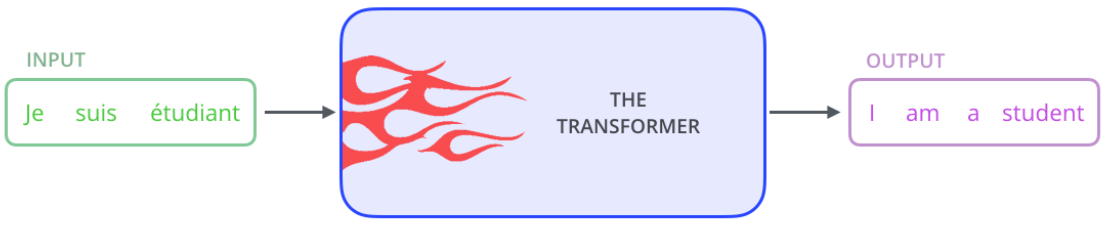
\includegraphics[width=\textwidth]{images/transormers.png}
    \caption{Transformers.}
    \label{fig:transformers}
\end{figure}

\begin{figure}
    \centering
    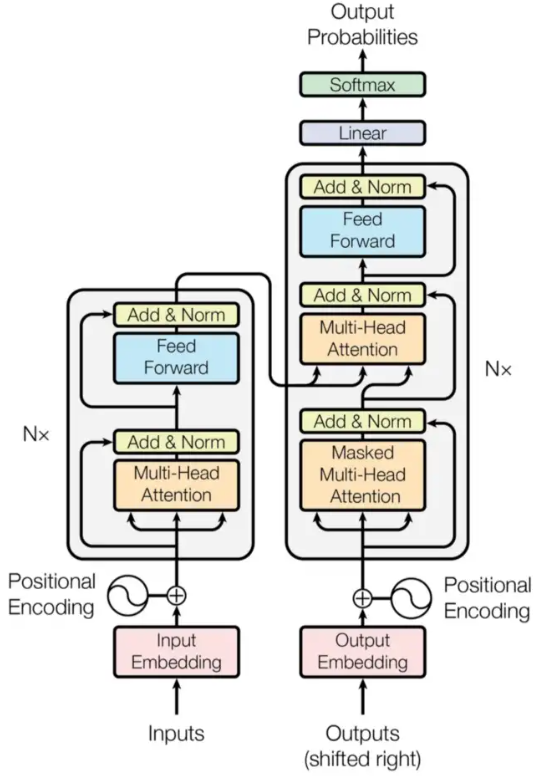
\includegraphics[width=\textwidth]{images/transformerMedium.png}
    \caption{The Transformer model architecture.}
    \label{fig:transformerMedium}
\end{figure}

\begin{figure}
    \centering
    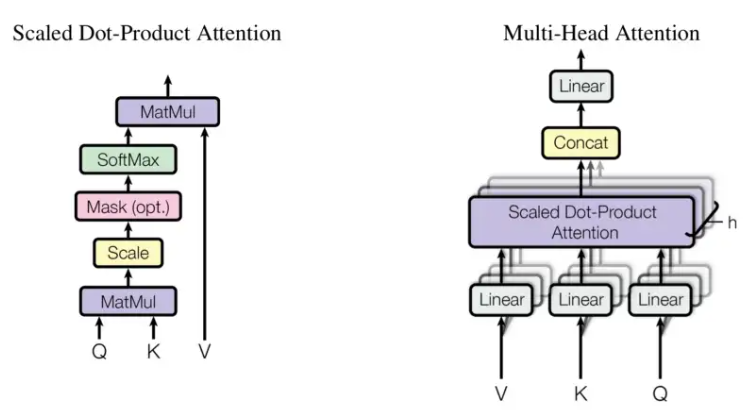
\includegraphics[width=\textwidth]{images/multiHeadAttentionBricks.png}
    \caption{(left) Scaled Dot-Product Attention. (right) Multi-Head Attention consists of several attention layers running in parallel.}
    \label{fig:multiHeadAttentionBricks}
\end{figure}

\subsubsection{Inference}
Inferring with those models is different from the training, which makes sense because in the end we want to translate a French sentence without having the German sentence. The trick here is to re-feed our model for each position of the output sequence until we come across an end-of-sentence token. \newline

A more step by step method would be:
\begin{itemize}
    \item Input the full encoder sequence (French sentence) and as decoder input, we take an empty sequence with only a start-of-sentence token on the first position. This will output a sequence where we will only take the first element.
    
    \item That element will be filled into second position of our decoder input sequence, which now has a start-of-sentence token and a first word/character in it.
    
    \item Input both the encoder sequence and the new decoder sequence into the model. Take the second element of the output and put it into the decoder input sequence.
    
    \item Repeat this until you predict an end-of-sentence token, which marks the end of the translation.
\end{itemize}

We see that we need multiple runs through our model to translate our sentence.

\subsubsection{Professor slide}
\begin{itemize}
    \item Use attention mechanism to learn input word encodings that depend on other words in the sentence
    
    \item Use attention mechanism to learn output word encodings that depend on input word encodings and previously generated output words
    
    \item Predict output words sequentially stopping when the "word" end-of-sentence is predicted
\end{itemize}

\subsection{Graph Neural Networks}
At this point we understood that deep learning is good at capturing hidden patterns of Euclidean data (images, text, videos). But what about applications where data is generated from non-Euclidean domains, represented as graphs with complex relationships and interdependencies between objects? That’s where \textit{Graph Neural Networks} (GNN) come in, which we’ll explore in this subsection (Figure \ref{fig:graph_neural_networks}). \newline

Sometimes the nodes of the represented graph have a set of features (for example, a user profile). If the node has $f$ numbers of features, then the node feature matrix $X$ has a dimension of ($n \times f$). \newline

Graph data is so complex that it’s created a lot of challenges for existing machine learning algorithms (Figure \ref{fig:networksVsImages}). \newline

The reason is that conventional Machine Learning and Deep Learning tools are specialized in simple data types. Like images with the same structure and size, which we can think of as fixed-size grid graphs. Text and speech are sequences, so we can think of them as line graphs. \newline

But there are more complex graphs, without a fixed form, with a variable size of unordered nodes, where nodes can have different amounts of neighbors. \newline

It also doesn’t help that existing machine learning algorithms have a core assumption that instances are independent of each other. This is false for graph data, because each node is related to others by links of various types. \newline

Graph Neural Networks (GNNs) are a class of deep learning methods designed to perform inference on data described by graphs. \newline

GNNs are neural networks that can be directly applied to graphs, and provide an easy way to do node-level, edge-level, and graph-level prediction tasks.\newline

GNNs can do what Convolutional Neural Networks (CNNs) failed to do. \newline

CNNs can be used to make machines visualize things, and perform tasks like image classification, image recognition, or object detection. This is where CNNs are the most popular. \newline

The core concept behind CNNs introduces hidden convolution and pooling layers to identify spatially localized features via a set of receptive fields in kernel form (Figure \ref{fig:cnnOnAnImage}). \newline

How does convolution operate on images that are regular grids? We slide the convolutional operator window across a two-dimensional image, and we compute some function over that sliding window. Then, we pass it through many layers. \newline

Our goal is to generalize the notion of convolution beyond these simple two-dimensional lattices. \newline

The insight allowing us to reach our goal is that convolution takes a little sub-patch of the image (a little rectangular part of the image), applies a function to it, and produces a new part (a new pixel). \newline

What happens is that the center node of that center pixel aggregates information from its neighbors, as well as from itself, to produce a new value. \newline

It’s very difficult to perform CNN on graphs because of the arbitrary size of the graph, and the complex topology, which means there is no spatial locality. \newline

There’s also unfixed node ordering. If we first labeled the nodes A, B, C, D, E, and the second time we labeled them B, D, A, E, C, then the inputs of the matrix in the network will change. Graphs are invariant to node ordering, so we want to get the same result regardless of how we order the nodes. \newline

In graph theory, we implement the concept of Node Embedding. It means mapping nodes to a d- dimensional embedding space (low dimensional space rather than the actual dimension of the graph), so that similar nodes in the graph are embedded close to each other. \newline

Our goal is to map nodes so that similarity in the embedding space approximates similarity in the network.  \newline

Let’s define $u$ and $v$ as two nodes in a graph.  \newline

$x_u$ and $x_v$ are two feature vectors. \newline

Now we’ll define the encoder function $\text{Enc}(u)$ and $\text{Enc}(v)$, which converts the feature vectors to $z_u$ and $z_v$ (Figure \ref{fig:fromInputNetworkToEmbeddingSpace}). \newline

Note: the similarity function could be Euclidean distance. \newline

So the challenge now is how to come up with the encoder function? \newline

The encoder function should be able to perform : \newline

\begin{itemize}
    \item Locality (local network neighborhoods)
    
    \item Aggregate information
    
    \item Stacking multiple layers (computation)
\end{itemize}

Locality information can be achieved by using a \textit{computational graph}. As shown in the graph of Figure \ref{fig:computationalGraph}, $i$ is the red node where we see how this node is connected to its neighbors and those neighbors’ neighbors. We’ll see all the possible connections, and form a computation graph. \newline

By doing this, we’re capturing the structure, and also borrowing feature information at the same time. \newline

Once the locality information preserves the computational graph, we start aggregating. This is basically done using neural networks (Figure \ref{fig:computationalGraphNeuralNetwork}). \newline

Neural Networks are presented in grey boxes. They require aggregations to be order-invariant, like sum, average, maximum, because they are permutation-invariant functions. This property enables the aggregations to be performed. \newline

Let’s move on to the forward propagation rule in GNNs. It determines how the information from the input will go to the output side of the neural network (Figure \ref{fig:computationalGraphNeuralNetwork1}). \newline

Every node has a feature vector. \newline

For example, ($X_A$) is a feature vector of node $A$. \newline

The inputs are those feature vectors, and the box will take the two feature vectors ($X_A$ and $X_c$), aggregate them, and then pass on to the next layer. \newline

Notice that, for example, the input at node $C$ are the features of node $C$, but the representation of node $C$ in layer 1 will be a hidden, latent representation of the node, and in layer 2 it’ll be another latent representation. \newline

Now, to train the model we need to define a loss function on the embeddings. We can feed the embeddings into any loss function and run stochastic gradient descent to train the weight parameters. Training can be unsupervised or supervised.

\begin{figure}[H]
    \centering
    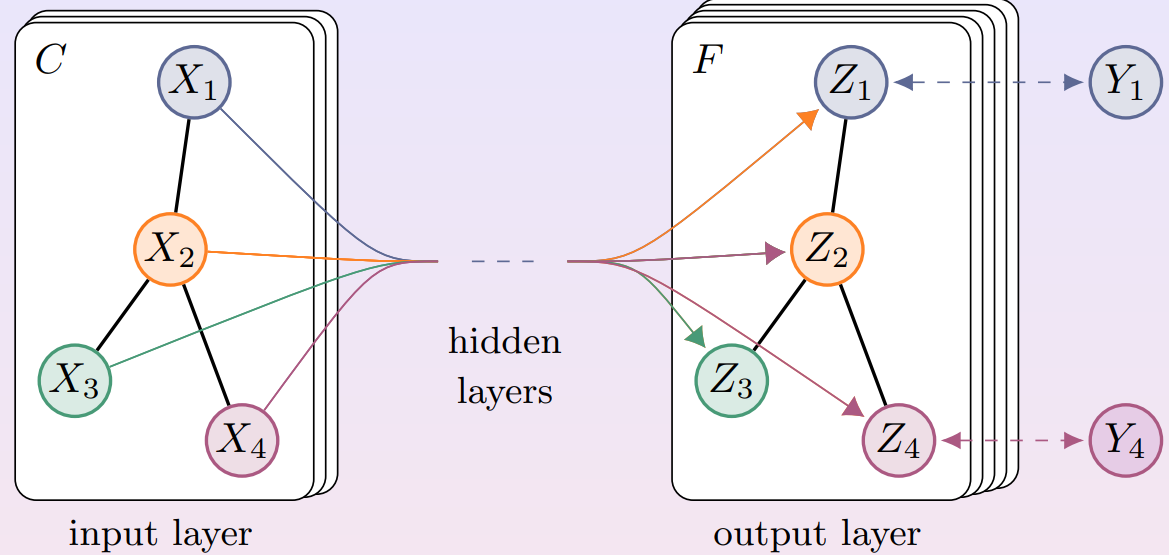
\includegraphics[width=\textwidth]{images/graphNeuralNetworl.png}
    \caption{Graph Neural Networks.}
    \label{fig:graph_neural_networks}
\end{figure}

\begin{figure}[H]
    \centering
    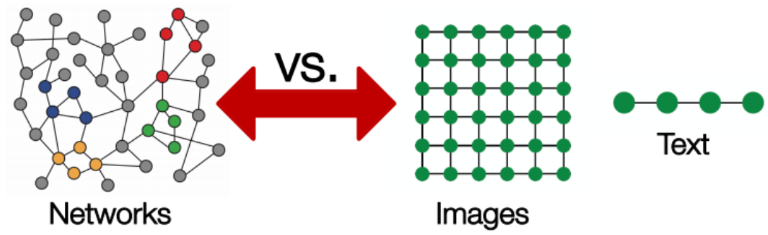
\includegraphics[width=\textwidth]{images/networksVsImages.png}
    \caption{Conventional Machine Learning and Deep Learning tools are specialized in simple data types. Like images with the same structure and size, which we can think of as fixed-size grid graphs. Text and speech are sequences, so we can think of them as line graphs.}
    \label{fig:networksVsImages}
\end{figure}

\begin{figure}[H]
    \centering
    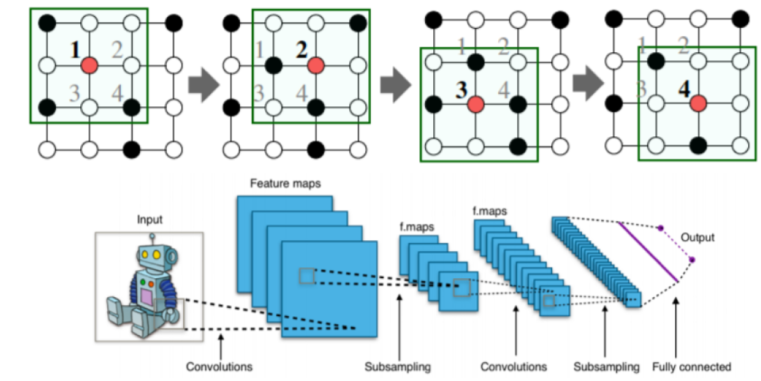
\includegraphics[width=\textwidth]{images/cnnOnAnImage.png}
    \caption{The core concept behind CNNs introduces hidden convolution and pooling layers to identify spatially localized features via a set of receptive fields in kernel form.}
    \label{fig:cnnOnAnImage}
\end{figure}

\begin{figure}[H]
    \centering
    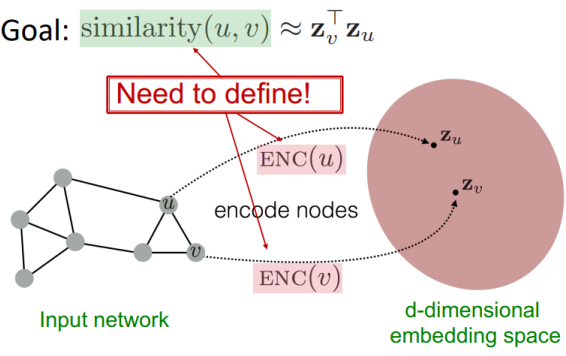
\includegraphics[width=\textwidth]{images/fromInputNetworkToEmbeddingSpace.png}
    \caption{The encoder function $\text{Enc}(u)$ and $\text{Enc}(v)$, converts the feature vectors to $z_u$ and $z_v$.}
    \label{fig:fromInputNetworkToEmbeddingSpace}
\end{figure}

\begin{figure}[H]
    \centering
    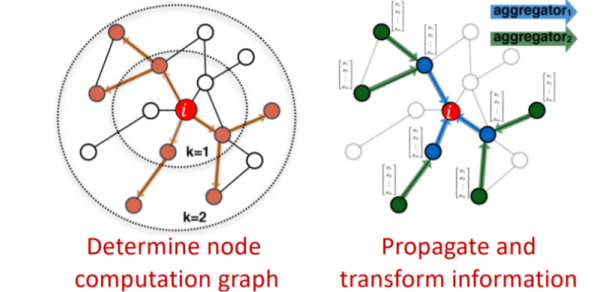
\includegraphics[width=\textwidth]{images/computationalGraph.png}
    \caption{Locality information can be achieved by using a \textit{computational graph}.}
    \label{fig:computationalGraph}
\end{figure}

\begin{figure}[H]
    \centering
    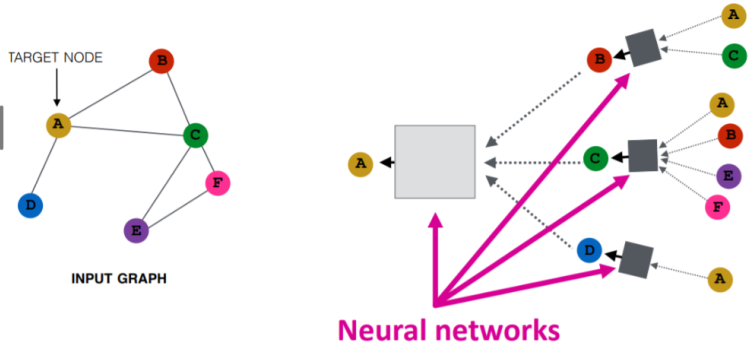
\includegraphics[width=\textwidth]{images/computationalGraphNeuralNetwork.png}
    \caption{Once the locality information preserves the computational graph, we start aggregating. This is basically done using neural networks.}
    \label{fig:computationalGraphNeuralNetwork}
\end{figure}

\begin{figure}[H]
    \centering
    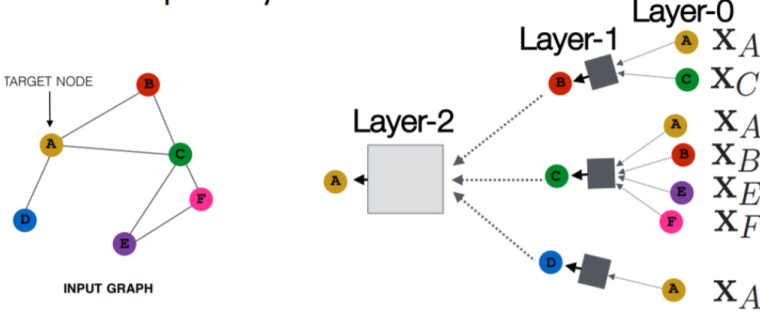
\includegraphics[width=\textwidth]{images/computationalGraphNeuralNetwork1.png}
    \caption{The forward propagation rule in GNNs. It determines how the information from the input will go to the output side of the neural network.}
    \label{fig:computationalGraphNeuralNetwork1}
\end{figure}

\subsubsection{Graph Convolutional Networks}
GCNs were first introduced in "Spectral Networks and Deep Locally Connected Networks on Graphs" (Bruna et al, 2014), as a method for applying neural networks to graph-structured data.

The simplest GCN has only three different operators:
\begin{itemize}
    \item Graph convolution 
    \item Linear layer 
    \item Nonlinear activation
\end{itemize}
The operations are usually done in this order. Together, they make up one network layer. We can combine one or more layers to form a complete GCN.

\subsubsection{Applications of GNNs}
Graph-structured data is present everywhere. The problems that GNNs resolve can be classified into these categories:

\begin{enumerate}
    \item Node Classification: the task here is to determine the labeling of samples (represented as nodes) by looking at the labels of their neighbors. Usually, problems of this type are trained in a semi-supervised way, with only a part of the graph being labeled.
    
    \item Graph Classification: the task here is to classify the whole graph into different categories. It’s like image classification, but the target changes into the graph domain. The applications of graph classification are numerous and range from determining whether a protein is an enzyme or not in bioinformatics, to categorizing documents in NLP, or social network analysis.
    
    \item Graph visualization: is an area of mathematics and computer science, at the intersection of geometric graph theory and information visualization. It is concerned with the visual representation of graphs that reveals structures and anomalies that may be present in the data and helps the user to understand the graphs.
    
    \item Link prediction: here, the algorithm has to understand the relationship between entities in graphs, and it also tries to predict whether there’s a connection between two entities. It’s essential in social networks to infer social interactions or to suggest possible friends to the users. It has also been used in recommender system problems and in predicting criminal associations.
    
    \item Graph clustering:  refers to the clustering of data in the form of graphs. There are two distinct forms of clustering performed on graph data. Vertex clustering seeks to cluster the nodes of the graph into groups of densely connected regions based on either edge weights or edge distances. The second form of graph clustering treats the graphs as the objects to be clustered and clusters these objects based on similarity. 
\end{enumerate}

\subsubsection{Professor slide}
Task: learning with graph convolution (Figure \ref{fig:graph_neural_networks}):
\begin{itemize}
    \item Allow to learn feature representations for nodes
    
    \item Allow to propagate information between neighbouring nodes
    
    \item Allow for efficient training (with respect to e.g. graph kernels)
\end{itemize}





